%% chapter9_slides.tex
%% Beamer slides for Chapter 9: Bayesian Detection of Unauthorized Expenditure
%% Using Langevin and Hamiltonian Monte Carlo
%% Bayesian Machine Learning in Quantitative Finance: Theory and Practical
%% Applications, Mongwe, Mbuvha & Marwala (Springer, 2025)
%% Compiled with: pdflatex -interaction=nonstopmode chapter9_slides.tex  (twice)
\documentclass[aspectratio=169,10pt]{beamer}

\usetheme{Madrid}
\usecolortheme{seahorse}
\usefonttheme{professionalfonts}

%% ── Packages ──────────────────────────────────────────────────────────────
\usepackage{amsmath,amssymb,amsfonts}
\usepackage{mathtools}
\usepackage{graphicx}
\usepackage{booktabs}
\usepackage{xcolor}
\usepackage{listings}
\usepackage{tikz}
\usetikzlibrary{arrows.meta,positioning,shapes.geometric,fit,backgrounds}

\graphicspath{{figures/}}

%% ── Python listing style ─────────────────────────────────────────────────
\lstdefinestyle{pycode}{
  language=Python,
  basicstyle=\ttfamily\scriptsize,
  numbers=left,
  numberstyle=\tiny\color{gray},
  frame=single,
  backgroundcolor=\color{gray!7},
  keywordstyle=\color{blue!70!black}\bfseries,
  commentstyle=\color{green!50!black}\itshape,
  stringstyle=\color{orange!80!black},
  showstringspaces=false,
  breaklines=true,
  tabsize=4,
  xleftmargin=1.5em,
  framexleftmargin=1.5em,
  aboveskip=4pt,
  belowskip=4pt,
}
\lstset{style=pycode}

%% ── Metadata ─────────────────────────────────────────────────────────────
\title[Bayesian ML in QF -- Ch.9]{Bayesian Machine Learning in Quantitative Finance}
\subtitle{Chapter 9: Detecting Unauthorized Expenditure}
\author{Based on Mongwe, Mbuvha \& Marwala}
\institute{Langevin and Hamiltonian Monte Carlo for Public-Finance Oversight}
\date{Springer, 2025}

\setbeamertemplate{footline}[frame number]
\setbeamertemplate{navigation symbols}{}

%% Helpful macros
\newcommand{\vw}{\mathbf{w}}
\newcommand{\vp}{\mathbf{p}}
\newcommand{\vx}{\mathbf{x}}
\newcommand{\R}{\mathbb{R}}
\newcommand{\E}{\mathbb{E}}
\newcommand{\Prob}{\mathbb{P}}

%% ══════════════════════════════════════════════════════════════════════════
\begin{document}

%% ── Title frame ──────────────────────────────────────────────────────────
\begin{frame}
  \titlepage
\end{frame}

%% ── Outline ──────────────────────────────────────────────────────────────
\begin{frame}{Chapter Overview}
  \tableofcontents
\end{frame}

%% ══════════════════════════════════════════════════════════════════════════
\section{9.1 Introduction}
%% ══════════════════════════════════════════════════════════════════════════

\begin{frame}[allowframebreaks]{9.1 Introduction: Why Municipal Overspending Matters}

\textbf{Intuition first.} A municipality has a legally approved budget. If it
spends money that was never authorized in that budget -- or spends a
conditional grant on something other than what it was earmarked for -- that
spending is a compliance failure, independent of whether anyone stole
anything. Detecting this \emph{before} the annual audit is a genuine
public-finance oversight problem, and it is exactly the kind of
structured-data classification problem where Bayesian machine learning can
help.

\begin{block}{The South African context}
The Auditor-General of South Africa (AGSA) found that \textbf{68\% of
municipalities} expended \textbf{R25.47 billion} in unauthorized spending in
the 2021--2022 fiscal year. South Africa has 257 municipalities (8
metropolitan, 44 district, 205 local), constitutionally mandated to deliver
services such as water, sanitation, power, roads, and refuse collection --
funded partly through own revenue and partly through conditional/unconditional
grants from provincial and national government.
\end{block}

\framebreak

\begin{block}{What this chapter does}
\begin{itemize}
  \item Builds a \textbf{Bayesian logistic regression} model that predicts,
  from a municipality's \emph{unaudited} financial ratios, whether its
  \emph{audited} statements will later be flagged for unauthorized
  expenditure.
  \item Trains this model with four MCMC samplers: MH, MALA, HMC, and
  \textbf{Magnetic HMC (MHMC)} -- the new method introduced in this chapter.
  \item Uses an automatic relevance determination (ARD) prior so the model
  also \emph{ranks which financial ratios matter most} -- useful for
  auditors deciding where to focus limited audit resources.
\end{itemize}
\end{block}

\textbf{Why this matters for risk-based auditing:} previous work
(Sikhosana, 2021) only established statistical \emph{correlations} between
unlawful spending and financial ratios computed from the \emph{same} audited
statements as the target -- i.e., it could not be used before the audit was
performed. This chapter is presented as the first-in-literature attempt to
\emph{predict} unauthorized expenditure using only unaudited (pre-audit)
financials, turning this into a genuine risk-screening tool.

\end{frame}

%% ══════════════════════════════════════════════════════════════════════════
\section{9.2 Background to Unlawful Expenditure}
%% ══════════════════════════════════════════════════════════════════════════

\begin{frame}[allowframebreaks]{9.2 Background to Unlawful Expenditure Analysis}

\textbf{Intuition.} South Africa's Public Finance Management Act (PFMA, 1999)
requires government entities to spend efficiently and within budget. When
the Auditor-General reviews a municipality's books, any spending that
breaks these rules is labeled \emph{unlawful}, and it comes in four flavors.

\begin{block}{Four categories of unlawful expenditure}
\begin{itemize}
  \item \textbf{Unauthorized expenditure:} money spent that was not budgeted
  for, or that did not match the terms of a grant. \emph{(The focus of this
  chapter.)}
  \item \textbf{Irregular expenditure:} spending not incurred in the manner
  required by law -- does \emph{not} always imply money was wasted or fraud
  occurred, just that the correct procurement/process rules were not
  followed.
  \item \textbf{Fruitless and wasteful expenditure:} spending made in vain
  that reasonable care could have avoided.
  \item \textbf{Irregular, wasteful, fruitless \& unauthorized} are
  collectively termed \textbf{unlawful expenditure}.
\end{itemize}
\end{block}

\framebreak

\begin{block}{Why financial ratios should help}
Sikhosana (2021) found statistically significant relationships between
unlawful spending and financial-performance ratios: e.g., a
\emph{negative} link between unauthorized expenditure and current ratio,
cost coverage, and net operating surplus margin. This tells us the ratios
carry signal -- but that analysis only described correlations \emph{after
the fact}, using ratios computed from the audited statements themselves
(the same source as the label). That is not useful as an early-warning
tool.
\end{block}

\begin{block}{This chapter's contribution}
Use a \textbf{Bayesian} approach for two reasons: (1) it gives
probabilistically sound predictions with \textbf{uncertainty bounds}, not
just point classifications; (2) an ARD-style prior gives a natural
\textbf{importance ranking} of the input ratios, which is directly
interpretable to auditors deciding where to allocate limited audit
resources.
\end{block}

\end{frame}

%% ══════════════════════════════════════════════════════════════════════════
\section{Recap: MH, MALA, HMC (brief)}
%% ══════════════════════════════════════════════════════════════════════════

\begin{frame}[allowframebreaks]{Notation You'll Need / Efficient Recap}

You have already seen MH, MALA and HMC in earlier chapters of this series
(Ch.\,3, Ch.\,7). Here is the compressed recap before we introduce what's
\textbf{new} in this chapter: Magnetic HMC.

\begin{block}{Metropolis--Hastings (MH) -- one line}
Propose $\vw^\ast \sim \mathcal{N}(\vw, \sigma^2 I)$ (a symmetric random
walk around the current state), accept with probability
$\min\!\big(1, \tfrac{p(\vw^\ast|\mathrm D)}{p(\vw|\mathrm D)}\big)$. No
gradient information is used, so proposals are unaware of which direction
improves the posterior -- this produces highly autocorrelated chains that
need very large sample sizes.
\end{block}

\begin{block}{MALA -- Langevin dynamics + MH correction}
$$ d\vw_t = \tfrac{1}{2} f'(\vw) \, dt + dZ_t \qquad (9.3)$$
where $f(\vw)$ is the target log-posterior, $f'(\vw)$ is its first
derivative (the drift, pulling proposals \emph{uphill}), and $Z_t$ is
Brownian motion (the diffusive/exploratory part). Discretizing with
Euler--Maruyama introduces error, so a Metropolis accept/reject step is
added on top to guarantee the correct stationary distribution. MALA mixes
faster than MH because the drift term exploits gradient information, but
samples are still noticeably correlated.

\framebreak
\end{block}

\begin{block}{HMC -- Hamiltonian dynamics}
Introduce an auxiliary momentum $\vp$ and simulate a physical system with
Hamiltonian $H(\vw,\vp) = -\log p(\vw|\mathrm D) + \tfrac12\vp^{\!\top} M^{-1}\vp$
(potential energy = negative log-posterior, kinetic energy = Gaussian in
$\vp$):
$$ \frac{d\vw}{dt} = \frac{\partial H(\vw,\vp)}{\partial \vp}\,, \qquad
   \frac{d\vp}{dt} = -\frac{\partial H(\vw,\vp)}{\partial \vw} \qquad (9.4)$$
Integrated numerically with the \textbf{leapfrog} scheme, then corrected
with a Metropolis accept step to cancel discretization error. Because HMC
proposes distant, high-acceptance-probability points by following the
energy-conserving trajectory, its samples are far less autocorrelated than
MH or MALA. When the trajectory length is set to 1 leapfrog step, HMC
reduces exactly to MALA.
\end{block}

\framebreak

\begin{block}{What's new: Magnetic Hamiltonian Monte Carlo (MHMC) -- plain-language intuition}
Ordinary HMC is a \textbf{marble rolling under gravity/potential forces
alone}: at every point it only feels the pull of the landscape
(the gradient of the negative log-posterior), so it swings back and forth
along smooth, in-plane arcs.

\medskip
\textbf{Magnetic HMC adds an extra force that always pushes sideways --
perpendicular to the current direction of motion} -- exactly like the
Lorentz force on a charged particle moving through a magnetic field. A
sideways force cannot speed a particle up or slow it down (it does no
work), but it \emph{bends} the path. This breaks the usual symmetric,
purely-gradient-driven HMC trajectory in a controlled, still-valid way, and
for some posteriors (especially ones with correlated or curved geometry)
the resulting curving/spiraling exploration mixes faster than straight HMC
sweeps.
\end{block}

\end{frame}

%% ══════════════════════════════════════════════════════════════════════════
\section{9.3 Model for Bayesian Detection of Expenditure}
%% ══════════════════════════════════════════════════════════════════════════

\begin{frame}[allowframebreaks]{9.3 Model for Bayesian Detection of Expenditure}

\textbf{Intuition.} We want a probabilistic yes/no classifier: given a
municipality's unaudited financial ratios, what is the probability that its
statements will show unauthorized expenditure? A \textbf{Bayesian logistic
regression} is the natural choice: logistic regression handles the
binary classification, and the Bayesian treatment gives us calibrated
uncertainty plus automatic feature-importance ranking.

\begin{block}{Negative log-likelihood (Eq.\,9.1)}
$$ l(\mathrm D|\vw) = \sum_{i}^{N} y_i \log(\vw^{\!\top} x_i) + (1-y_i)\log(1-\vw^{\!\top} x_i) $$
where $\mathrm D = \{\vx, \vy\}$ is the data, $N$ is the number of
observations, $\vw$ are the parameters (regression weights) to be
estimated, $y_i \in \{0,1\}$ is the unauthorized-expenditure label for
observation $i$, and $x_i$ is its feature vector of financial ratios.
(In practice $\vw^{\!\top} x_i$ is passed through a sigmoid link so it lies
in $(0,1)$ before being interpreted as a probability.)
\end{block}

\framebreak

\begin{block}{Un-normalized log-posterior (Eq.\,9.2)}
$$ \ln p(\vw|\mathrm D) = l(\mathrm D|\vw) + \ln p(\vw|\alpha) + \ln q(\alpha) $$
where $\ln p(\vw|\alpha)$ is the log-prior on the weights given
hyperparameters $\alpha$, and $\ln q(\alpha)$ is the distribution placed on
those hyperparameters. This is the un-normalized target that every MCMC
sampler in this chapter (MH, MALA, HMC, MHMC) draws samples from.
\end{block}

\begin{block}{Automatic Relevance Determination (ARD) prior}
Each weight $w_i$ has \textbf{its own} Gaussian prior, zero mean, with its
own standard deviation/regularization parameter $\alpha_i$. Large $\alpha_i$
$\Rightarrow$ feature $i$ is important (its weight is free to move far from
zero); $\alpha_i \to 0$ $\Rightarrow$ feature $i$ is irrelevant (its weight
is shrunk to zero). This automatically ranks feature importance as a
by-product of inference -- no separate feature-selection step needed.
The $\alpha_i$ are themselves given a log-normal distribution (mean 0, unit
variance), and $\vw$ and $\alpha$ are sampled \emph{jointly} rather than via
a Gibbs step -- this doubles the effective parameter space but gives more
stable MCMC exploration in practice.
\end{block}

\framebreak

\begin{block}{Why joint sampling instead of Gibbs sampling for $\alpha$?}
An alternative (Neal, 2012) alternates HMC for the weights $\vw$ with Gibbs
sampling of $\alpha$ from a Gamma posterior. This converges to the
asymptotically correct joint posterior, but still requires design choices
(e.g. the exact conjugate prior family). Jointly sampling $\vw$ and $\alpha$
with the log-normal parameterization avoids this extra design step and, per
the authors, gives more stable exploration -- at the cost of a doubled
parameter dimension for the sampler to explore.
\end{block}

\end{frame}

\begin{frame}[fragile]{Python: Bayesian Logistic Regression with an ARD Prior}
\begin{lstlisting}
import numpy as np

def sigmoid(z):
    return 1.0 / (1.0 + np.exp(-z))

def neg_log_likelihood(w, X, y):
    # Eq. 9.1: l(D|w) -- numerically stable form via log1p/logaddexp
    z = X @ w
    return -np.sum(y * (-np.logaddexp(0, -z))
                   + (1 - y) * (-np.logaddexp(0, z)))

def log_prior(w, alpha):
    # zero-mean Gaussian prior, one std dev alpha_i PER weight (ARD)
    return -0.5 * np.sum((w ** 2) / (alpha ** 2)) - np.sum(np.log(alpha))

def log_hyperprior(alpha):
    # alpha_i ~ LogNormal(mean=0, var=1)
    return -0.5 * np.sum(np.log(alpha) ** 2) - np.sum(np.log(alpha))

def log_posterior(w, alpha, X, y):
    # Eq. 9.2: joint (unnormalized) target for MCMC over (w, alpha)
    return (-neg_log_likelihood(w, X, y)
            + log_prior(w, alpha) + log_hyperprior(alpha))
\end{lstlisting}
\end{frame}

%% ══════════════════════════════════════════════════════════════════════════
\section{9.4 Markov Chain Monte Carlo Algorithms}
%% ══════════════════════════════════════════════════════════════════════════

\subsection{9.4.1 Metropolis-Hastings and MALA}

\begin{frame}[allowframebreaks]{9.4.1 Metropolis-Hastings and the Metropolis-Adjusted Langevin Algorithm}

\textbf{Intuition.} We now train the ARD Bayesian logistic regression model
above with four different samplers. MH and MALA are the efficient recap
(seen in previous chapters); the emphasis here is on how the book applies
them to \emph{this} expenditure-detection posterior.

\begin{block}{MH: the baseline}
Random-walk Metropolis-Hastings uses a Gaussian proposal centered at the
current state. It ignores gradient information entirely, so its
exploration is undirected -- in this chapter's results, MH indeed produces
the most highly autocorrelated samples of all four methods, and the lowest
predictive performance.
\end{block}

\begin{block}{MALA: adds first-order gradient information}
MALA improves on MH by using the drift term $\tfrac12 f'(\vw)$ (Eq.\,9.3)
to bias proposals \emph{uphill} in log-posterior, then Metropolis-corrects
for the discretization error of the Euler--Maruyama integration. This
directs exploration using local curvature (first-order gradient) rather
than undirected random-walk steps, so MALA converges faster and mixes
better than MH -- though its samples remain correlated relative to
Hamiltonian-based methods.
\end{block}

\framebreak

\begin{block}{A note on manifold extensions}
Riemannian-manifold variants of Langevin and Hamiltonian dynamics (Girolami
\& Calderhead, 2011) go further and use \emph{second}-order gradient
(curvature) information, at higher computational cost. In practice, methods
using Hamiltonian dynamics on the ordinary Euclidean manifold (as used in
this chapter) have shown great promise and are considerably simpler to
implement.
\end{block}

\end{frame}

\begin{frame}[fragile]{Python: From-Scratch MALA on the Toy Posterior}
\begin{lstlisting}
def grad_log_posterior(w, X, y):
    z = X @ w
    p = sigmoid(z)
    return X.T @ (y - p) - w / TAU**2   # analytic gradient (fixed-alpha case)

def run_mala(n_iter, step, w0, X, y, seed=1):
    rng = np.random.default_rng(seed)
    w = w0.copy()
    lp, grad = log_posterior(w, X, y), grad_log_posterior(w, X, y)
    chain, n_accept = np.zeros((n_iter, len(w))), 0
    for m in range(n_iter):
        mean_fwd = w + 0.5 * step * grad                # Eq. 9.3 drift
        prop = mean_fwd + np.sqrt(step) * rng.standard_normal(len(w))
        lp_prop = log_posterior(prop, X, y)
        grad_prop = grad_log_posterior(prop, X, y)
        mean_bwd = prop + 0.5 * step * grad_prop
        log_q_fwd = -np.sum((prop - mean_fwd) ** 2) / (2 * step)
        log_q_bwd = -np.sum((w - mean_bwd) ** 2) / (2 * step)
        log_alpha = (lp_prop + log_q_bwd) - (lp + log_q_fwd)   # MH correction
        if np.log(rng.uniform()) < log_alpha:
            w, lp, grad = prop, lp_prop, grad_prop
            n_accept += 1
        chain[m] = w
    return chain, n_accept / n_iter
\end{lstlisting}
\end{frame}

\subsection{9.4.2 HMC and Magnetic HMC}

\begin{frame}[allowframebreaks]{9.4.2 Hamiltonian Monte Carlo -- Efficient Recap}

\begin{block}{Leapfrog integration (Eq.\,9.5)}
$$ \vp_{t+\epsilon/2} = \vp_t + \frac{\epsilon}{2}\frac{\partial H(\vw_t,\vp_t)}{\partial \vw} $$
$$ \vw_{t+\epsilon} = \vw_t + \epsilon M^{-1} \vp_{t+\epsilon/2} $$
$$ \vp_{t+\epsilon} = \vp_{t+\epsilon/2} + \frac{\epsilon}{2}\frac{\partial H(\vw_{t+\epsilon},\vp_{t+\epsilon/2})}{\partial \vw} $$
where $\epsilon$ is the discretization step size and $M$ is the covariance
matrix of the (Gaussian) kinetic energy term. This is a symmetric
half-step/full-step/half-step split that approximately conserves $H$.
\end{block}

\begin{block}{Metropolis correction (Eq.\,9.6)}
$$ \Prob(\text{accept } \vw^\ast) = \min\!\left(1, \frac{\exp(-H(\vw^\ast,\vp^\ast))}{\exp(-H(\vw,\vp))}\right) $$
Needed because the leapfrog integrator is not exact -- this restores exact
detailed balance. HMC's two tunable parameters are the step size $\epsilon$
(usually tuned via dual averaging to hit a target acceptance rate) and the
trajectory length (number of leapfrog steps) -- a harder parameter to tune,
often set via schemes such as the No-U-Turn Sampler.
\end{block}

\framebreak

\begin{block}{Why HMC helps here}
By simulating energy-conserving Hamiltonian trajectories rather than
undirected or purely-gradient-biased single steps, HMC can propose
\textbf{distant} points in parameter space that are still likely to be
accepted. This is what drives its low autocorrelation -- and, per this
chapter's results, its best-in-class predictive performance on the real
municipal dataset.
\end{block}

\end{frame}

\begin{frame}[allowframebreaks]{9.4.2 Magnetic Hamiltonian Monte Carlo (MHMC)}

\textbf{Intuition, restated precisely.} MHMC adds a \textbf{magnetic field}
matrix $G$ to the force field already present in HMC. This makes MHMC more
flexible than HMC and promotes more efficient investigation of the
posterior by reducing autocorrelation in the produced samples -- \emph{if}
the magnetic field interacts favorably with the force field (e.g. if they
are close to orthogonal).

\begin{block}{Non-canonical Hamiltonian dynamics (Eq.\,9.7)}
$$ \frac{d}{\partial t}\begin{bmatrix}\vw\\ \vp\end{bmatrix}
   = \begin{bmatrix} 0 & I \\ -I & G\end{bmatrix}
     \begin{bmatrix}\nabla_{\vw} H(\vw,\vp)\\ \nabla_{\vp} H(\vw,\vp)\end{bmatrix} $$
where $G$ is a \textbf{skew-symmetric} (antisymmetric) matrix, i.e.
$G^{\!\top} = -G$, and is the term that represents the magnetic field. The
Hamiltonian $H$ itself is \textbf{identical} to the one used in ordinary
HMC -- only the matrix multiplying the gradient changes.
\end{block}

\framebreak

\begin{block}{Step-by-step: exactly what changes vs.\ ordinary HMC}
Writing out both block rows of Eq.\,9.7 and comparing to Eq.\,9.4:
\begin{itemize}
  \item \textbf{Position update (unchanged):}
  $\dfrac{d\vw}{dt} = \nabla_{\vp} H(\vw,\vp)$ -- identical in HMC and MHMC.
  \item \textbf{Momentum update (this is where the new term enters):}
  \begin{align*}
    \text{HMC:}  &\quad \dfrac{d\vp}{dt} = -\nabla_{\vw} H(\vw,\vp) \\
    \text{MHMC:} &\quad \dfrac{d\vp}{dt} = -\nabla_{\vw} H(\vw,\vp) \; + \; G\,\nabla_{\vp} H(\vw,\vp)
  \end{align*}
\end{itemize}
The added term $G\,\nabla_{\vp} H(\vw,\vp)$ is exactly the extra
``sideways'' force: since $G$ is skew-symmetric, $\vp^{\!\top}(G\vp) = 0$,
so this term can never add or remove energy (it is orthogonal to $\vp$
itself) -- it can only \emph{redirect} the momentum. \textbf{HMC and MHMC
dynamics are identical whenever $G = 0$.}
\end{block}

\framebreak

\begin{block}{Setting the magnetic field $G$ (as done in this chapter)}
There is no general theory for how to choose $G$; the authors follow
Tripuraneni et al. (2017) and let only a \emph{few} dimensions interact with
the field. Concretely, for weight indices $1$ and $5$: $G_{1i} = G_{5i} = g$
and $G_{i1} = G_{i5} = -g$ for $g = 0.2$, zero elsewhere -- and $G$ is kept
anti-symmetric throughout. Like HMC, the resulting dynamics cannot be
integrated exactly, so a numerical integrator plus a Metropolis-Hastings
accept step is used to enforce detailed balance despite discretization
error.
\end{block}

\framebreak

\begin{block}{Physical analogy: Newtonian mechanics of a charged particle}
According to Tripuraneni et al. (2017), these non-canonical dynamics
represent the motion of a charged particle in a magnetic field in three
dimensions. The particle still feels the ordinary potential force
($-\nabla_{\vw}H$), but a magnetic-type Lorentz force
($G\,\nabla_{\vp}H$) bends its path sideways without changing its speed.
Whether MHMC actually samples \emph{more} efficiently than HMC on a given
posterior depends entirely on how this magnetic field geometrically
interacts with that posterior's force field -- there is no guarantee it
always helps, and (as we will see in Sect.\,9.6) it does not always help
in practice.
\end{block}

\end{frame}

\begin{frame}{Schematic: HMC vs.\ Magnetic HMC Trajectories (Toy 2D Potential)}
\begin{center}
  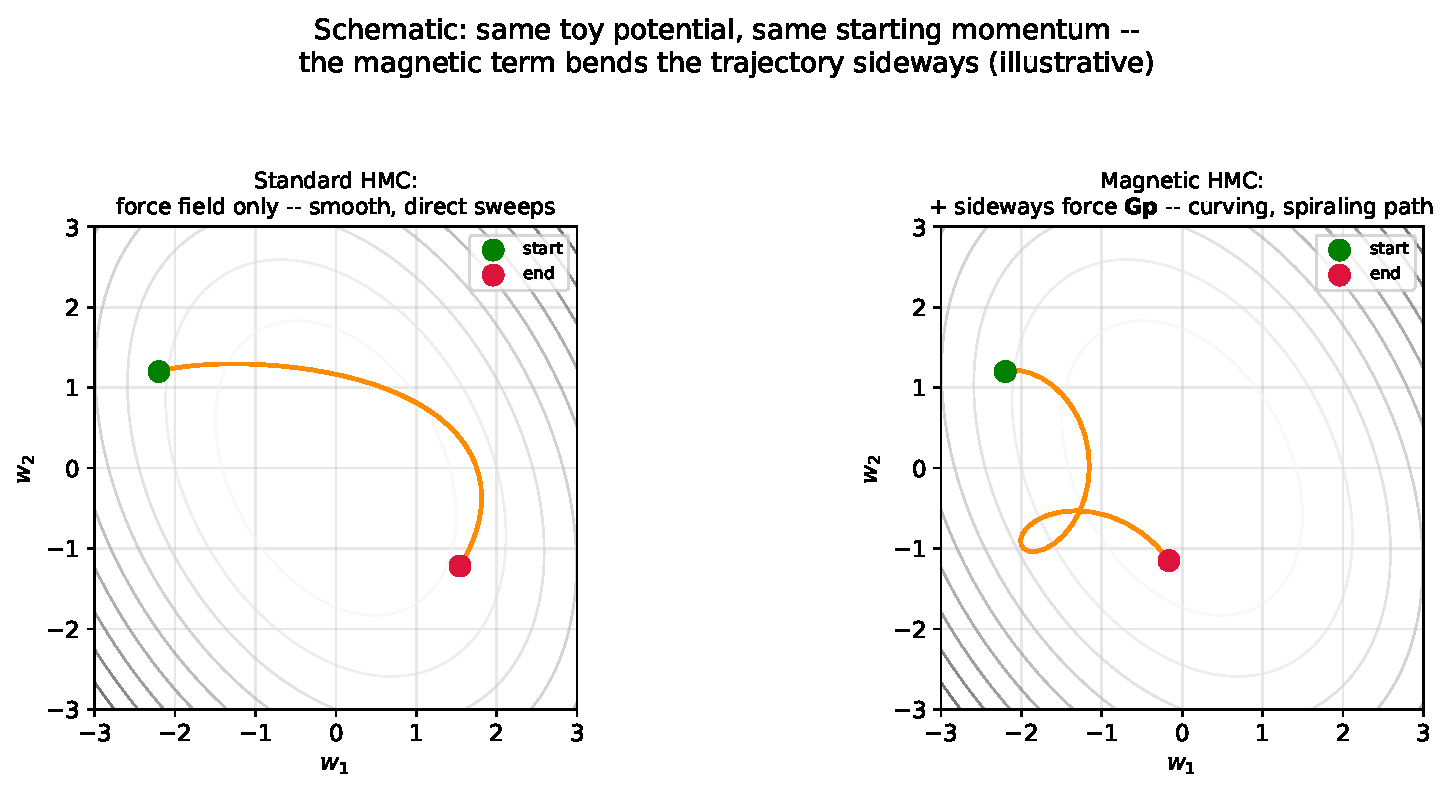
\includegraphics[width=0.98\textwidth]{fig_hmc_vs_mhmc_schematic.pdf}
\end{center}
{\scriptsize Illustrative toy quadratic potential, own simulation --
same starting position/momentum, same step size and number of leapfrog
steps. Left: ordinary HMC leapfrog (Eq.\,9.5) follows one smooth
gradient-driven arc. Right: adding the skew-symmetric $G$ term (Eq.\,9.7)
visibly curls the trajectory sideways, exactly like a charged particle
deflected by a magnetic field.}
\end{frame}

\begin{frame}[fragile]{Python: Leapfrog for HMC vs.\ Magnetic HMC (Toy Potential)}
\begin{lstlisting}
def grad_U(w, A):        # potential force: -grad(log posterior) = A @ w
    return A @ w

def leapfrog_hmc(w0, p0, eps, L, A):
    w, p = w0.copy(), p0.copy()
    for _ in range(L):
        p = p - 0.5 * eps * grad_U(w, A)     # HMC momentum half-step
        w = w + eps * p                       # position full-step
        p = p - 0.5 * eps * grad_U(w, A)     # HMC momentum half-step
    return w, p

def leapfrog_mhmc(w0, p0, eps, L, A, G):
    w, p = w0.copy(), p0.copy()
    for _ in range(L):
        force = -grad_U(w, A) + G @ p         # ADDED sideways term: G @ p
        p = p + 0.5 * eps * force
        w = w + eps * p
        force = -grad_U(w, A) + G @ p         # recompute with new w, p
        p = p + 0.5 * eps * force
    return w, p

# G must be skew-symmetric: G.T == -G  (e.g. G = [[0, g], [-g, 0]])
\end{lstlisting}
\end{frame}

%% ══════════════════════════════════════════════════════════════════════════
\section{Toy Running Example}
%% ══════════════════════════════════════════════════════════════════════════

\begin{frame}[allowframebreaks]{Toy Running Example: 6 Fictional Government Transactions}

\textbf{Purpose.} To make Sect.\,9.3--9.4 concrete, we build our own small,
fictional dataset in the same spirit as the book's real one, and fit the
ARD Bayesian logistic regression from scratch. \textbf{These numbers are
entirely illustrative} -- they are not from the book's real municipal
dataset.

\begin{table}
\centering
\scriptsize
\begin{tabular}{lllrrc}
\toprule
ID & Description & Department & Amount (R) & Budget var.\ (\%) & Label \\
\midrule
T1 & Roads resurfacing contract        & Infrastructure       & 850{,}000   & +12  & authorized \\
T2 & Emergency IT systems upgrade       & IT Services          & 4{,}200{,}000 & +145 & \textbf{unauthorized} \\
T3 & Community hall maintenance         & Community Services   & 310{,}000   & +5   & authorized \\
T4 & Bulk water pipeline repair         & Water \& Sanitation  & 2{,}600{,}000 & +88  & \textbf{unauthorized} \\
T5 & Office stationery supply           & Finance              & 190{,}000   & $-3$ & authorized \\
T6 & Unbudgeted road-signage project    & Roads \& Transport   & 3{,}100{,}000 & +110 & \textbf{unauthorized} \\
\bottomrule
\end{tabular}
\end{table}

Features used: standardized \emph{amount} ($x_1$) and standardized
\emph{budget-variance \%} ($x_2$) -- i.e. how far actual spend deviated
from the budgeted amount, our toy stand-in for the book's financial ratios.

\framebreak

\begin{center}
  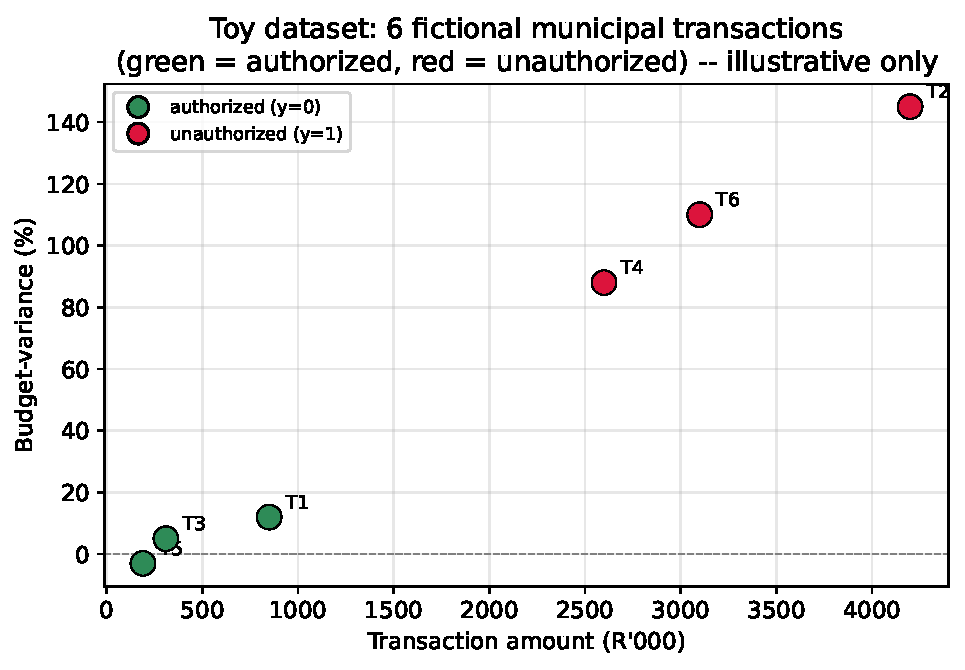
\includegraphics[width=0.72\textwidth]{fig_toy_data_scatter.pdf}
\end{center}
{\scriptsize Large, positive budget overruns coincide with unauthorized
labels in this toy example -- by design, since we made it up to be
illustrative of the intuition, not to be a subtle classification problem.}

\end{frame}

\begin{frame}[allowframebreaks]{Toy Running Example: Fitting the Model with MALA}

We fit the 3-parameter Bayesian logistic regression $w_0$ (intercept),
$w_1$ (amount coefficient), $w_2$ (budget-variance-\% coefficient) with
$\mathcal N(0,\tau^2)$ priors ($\tau=2$), using a from-scratch MALA sampler
(8{,}000 iterations, burn-in 1{,}500, step size tuned to $\approx$92\%
acceptance).

\begin{center}
  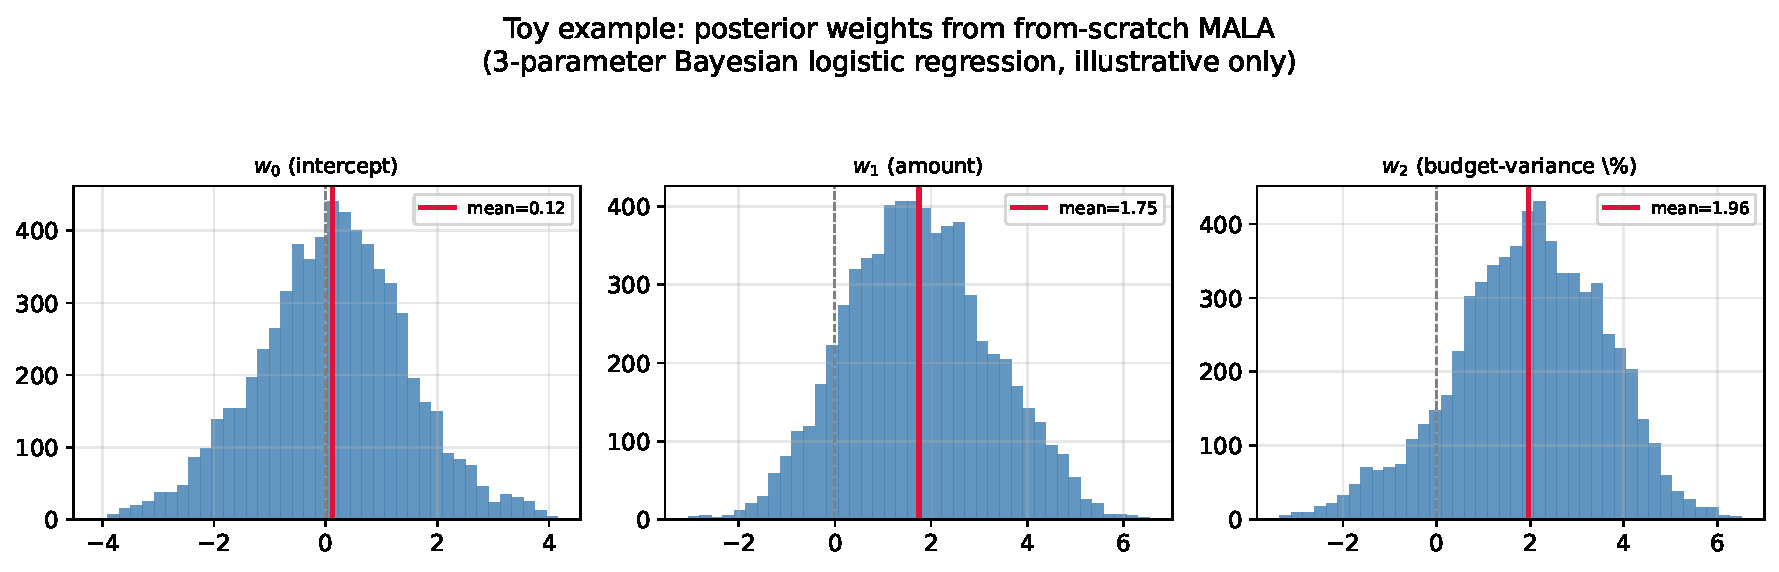
\includegraphics[width=0.98\textwidth]{fig_toy_posterior_summary.pdf}
\end{center}

\framebreak

\begin{block}{Illustrative posterior summary (own toy simulation)}
\begin{center}
\begin{tabular}{lcc}
\toprule
Parameter & Posterior mean & Posterior std.\ dev. \\
\midrule
$w_0$ (intercept)             & $0.12$ & $1.34$ \\
$w_1$ (amount)                 & $1.85$ & $1.62$ \\
$w_2$ (budget-variance \%)     & $1.97$ & $1.60$ \\
\bottomrule
\end{tabular}
\end{center}
Both $w_1$ and $w_2$ have posterior mass concentrated well away from zero
and of the same (positive) sign -- consistent with our toy design that
\emph{larger amounts and larger positive budget overruns} both push a
transaction towards ``unauthorized.'' With only 6 toy observations the
posterior is necessarily wide (large std.\ devs.) -- this is the Bayesian
framework being honest about how little data it has seen, exactly the
uncertainty quantification that a point-estimate classifier would hide.
\end{block}

\framebreak

\begin{block}{A new toy transaction}
For a new, unseen transaction of R2{,}000{,}000 with a $+60\%$ budget
variance, plugging the posterior mean weights into the sigmoid link gives
an illustrative $\Prob(\text{unauthorized}) \approx 0.57$ -- i.e. the toy
model is genuinely uncertain (just over a coin flip), which is a sensible
answer for a transaction that sits between the clearly-authorized and
clearly-unauthorized examples in our tiny training set.
\end{block}

\end{frame}

\begin{frame}{Toy Running Example: MH vs.\ MALA on the Same Sub-Posterior}
\begin{center}
  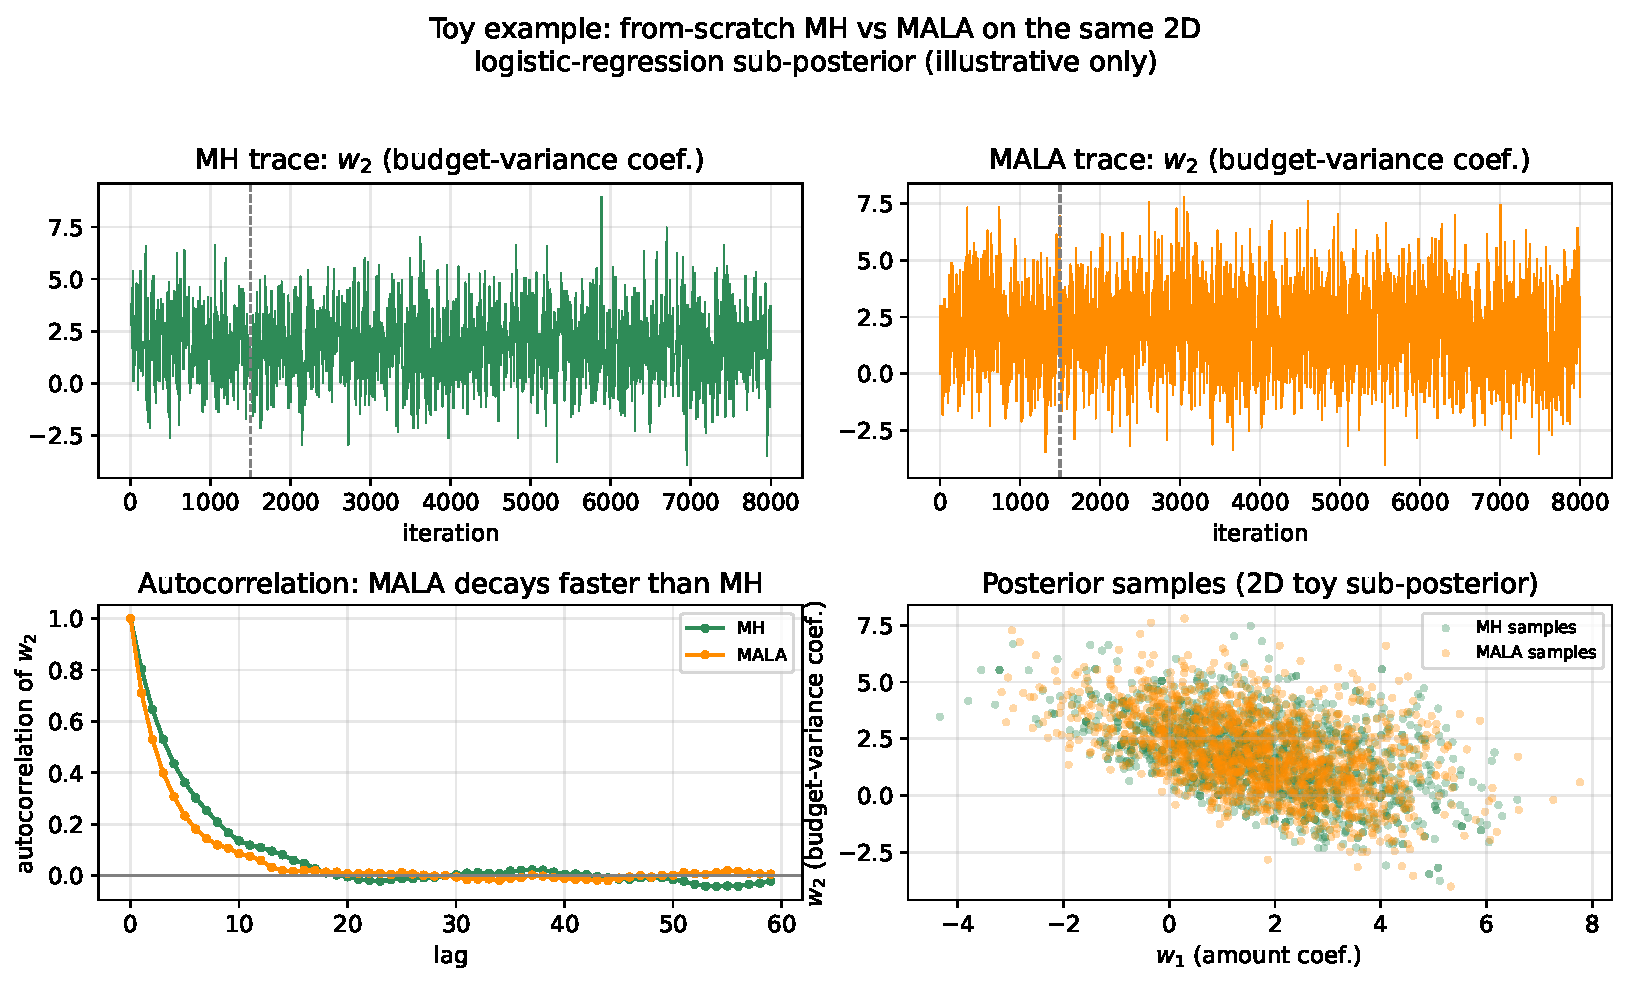
\includegraphics[width=0.98\textwidth]{fig_mh_vs_mala_toy.pdf}
\end{center}
{\scriptsize Own from-scratch simulation, illustrative only. MH proposal
tuned to $\approx$31\% acceptance, MALA to $\approx$83\%. MALA's
autocorrelation decays faster (bottom-left), giving a higher effective
sample size for the same 6{,}500 post-burn-in draws (rough ESS: MH
$\approx 663$ vs.\ MALA $\approx 905$) -- a small-scale echo of the
book's own finding that gradient-informed samplers beat plain MH.}
\end{frame}

%% ══════════════════════════════════════════════════════════════════════════
\section{9.5 Numerical Experiments}
%% ══════════════════════════════════════════════════════════════════════════

\subsection{9.5.1 Data Description}

\begin{frame}[allowframebreaks]{9.5.1 Data Description (the Book's Real Dataset)}

\begin{block}{Source and scope}
South African municipal finance dataset from the National Treasury website
(\texttt{municipaldata.treasury.gov.za}). \textbf{1{,}430 observations}
from 2012--2019, built from municipalities' \emph{unaudited} financial
statements as inputs, with the unauthorized-expenditure label taken from
the corresponding \emph{audited} financials.
\end{block}

\begin{block}{Eight financial-ratio features}
Debt to Community Wealth/Equity; Debt to Total Operating Revenue; Current
Ratio; Net Operating Surplus Margin \%; Remuneration \% of Total Operating
Expenditure; Contracted Services \% of Total Operating Expenditure; Net
Surplus/Deficit Water; Net Surplus/Deficit Electricity.
\end{block}

\framebreak

\begin{block}{Class balance and preprocessing}
When absolute expenditure amounts are converted to a binary label: 66\% of
observations have \emph{no} unauthorized expenditure, 34\% do. Data is
split 70/30 into train/test. The distribution of absolute expenditure
amounts is heavily right-skewed -- most municipalities have (near) zero
unauthorized expenditure, with a long tail of large violations, which is
exactly why this is framed as a \emph{binary detection} problem rather than
a regression on the Rand amount.
\end{block}

\end{frame}

\subsection{9.5.2 Experiment Description}

\begin{frame}{9.5.2 Experiment Description}

\begin{block}{Task}
Binary classification: does a given municipal financial report have
unauthorized expenditure? Encoded as $y=0$ (no) / $y=1$ (yes).
\end{block}

\begin{block}{Sampling setup}
10{,}000 MCMC samples generated per method, of which the first 5{,}000
form the burn-in (used for step-size tuning). Step sizes tuned via
primal-dual averaging (Hoffman \& Gelman) to hit target acceptance rates
of \textbf{25\% (MH), 60\% (MALA), 80\% (HMC and MHMC)}. Trajectory length
(number of leapfrog steps) for both HMC and MHMC fixed at \textbf{100}.
\end{block}

\end{frame}

\begin{frame}[fragile]{Python: Toy Experiment Harness (Same Structure as the Book)}
\begin{lstlisting}
# Illustrative harness mirroring the book's experimental protocol,
# applied to our toy 6-transaction dataset (NOT the book's real data).
N_SAMPLES, BURN_IN = 10_000, 5_000
TARGET_ACCEPT = {"MH": 0.25, "MALA": 0.60, "HMC": 0.80, "MHMC": 0.80}
TRAJECTORY_LENGTH = 100          # leapfrog steps, HMC and MHMC

def tune_step_size(sampler_fn, target_accept, X, y, **kwargs):
    """Simple bisection-style dual-averaging stand-in: adjust step until
    empirical acceptance rate is close to the target."""
    lo, hi = 1e-4, 5.0
    for _ in range(15):
        step = 0.5 * (lo + hi)
        _, acc = sampler_fn(n_iter=500, step=step, X=X, y=y, **kwargs)
        if acc > target_accept:
            lo = step          # accepted too often -> take bigger steps
        else:
            hi = step          # accepted too rarely -> take smaller steps
    return 0.5 * (lo + hi)
\end{lstlisting}
\end{frame}

\subsection{9.5.3 Performance Metrics for MCMC Methods}

\begin{frame}{9.5.3 Performance Metrics for MCMC Methods}

\begin{block}{Diagnostics used in the book}
\begin{itemize}
  \item \textbf{Trace plots} of the un-normalized target log-posterior.
  \item \textbf{Effective sample size (ESS)} -- the multivariate ESS
  measure of Vats et al. (2019), which accounts for autocorrelation across
  \emph{all} sampled dimensions jointly.
  \item \textbf{ESS normalized by execution time} -- ESS alone rewards
  cheap-but-slow-mixing methods unfairly; dividing by wall-clock time
  reveals which method delivers the most \emph{useful} samples per second.
  \item \textbf{Predictive performance}: Receiver Operating Characteristic
  (ROC) curve and Area Under the ROC (AUC) on held-out test data -- useful
  here because the relative cost of a false positive vs.\ a false negative
  audit flag is not clearly known in advance.
\end{itemize}
\end{block}

\end{frame}

%% ══════════════════════════════════════════════════════════════════════════
\section{9.6 Results and Discussion}
%% ══════════════════════════════════════════════════════════════════════════

\begin{frame}[allowframebreaks]{9.6 Results and Discussion}

\begin{block}{Effective sample size: HMC wins outright}
HMC produces the \textbf{highest} raw ESS, followed by MALA; MH and MHMC
both have low, similar ESS. On a \textbf{time-normalized} basis, however,
\textbf{MALA outperforms every method} -- its per-iteration cost is far
lower than the Hamiltonian-dynamics-driven methods, so despite mixing
somewhat slower per-sample than HMC, it delivers more effective samples per
second of compute. MH has the lowest execution time of all, followed by
MALA then HMC; \textbf{MHMC has the largest execution time} due to the
extra computation needed for the magnetic-field term.
\end{block}

\begin{block}{Why MHMC underperformed here}
All four methods converge (trace plots stabilize), but MHMC's poor ESS is
attributed to a \textbf{poor choice of the magnetic field for this
particular task} -- i.e. the fixed, hand-set $G$ (only coupling weights 1
and 5, with $g=0.2$) likely does not interact favorably with this
posterior's geometry. This points to the need to \emph{tune} $G$ rather
than fix it a priori.
\end{block}

\framebreak

\begin{block}{Predictive performance (test-set AUC)}
$$ \text{HMC: } 0.7108 \quad \text{MALA: } 0.7102 \quad
   \text{MHMC: } 0.7085 \quad \text{MH: } 0.6276 $$
HMC has the best predictive performance (highest AUC), which aligns with
its high effective sample size; MH has by far the poorest predictive
performance, tracking its very poor exploration of the posterior (visible
in its distinctly higher negative-log-likelihood trace and its inability
to escape a worse mode).
\end{block}

\begin{block}{Feature importance agreement}
The three gradient-informed methods (MALA, HMC, MHMC) broadly \textbf{agree}
on which financial ratios matter most, with \textbf{Current Ratio} and
\textbf{Debt to Total Operating Revenue} the most consistently top-ranked
features across methods -- consistent with earlier audit-outcome analyses
by the same authors. MH, lacking gradient information, cannot meaningfully
distinguish important from unimportant features (its posterior variances
for all 8 ratios come out similarly large).
\end{block}

\end{frame}

%% ══════════════════════════════════════════════════════════════════════════
\section{9.7 Conclusions}
%% ══════════════════════════════════════════════════════════════════════════

\begin{frame}{9.7 Conclusions}

\begin{block}{Summary}
\begin{itemize}
  \item First-in-literature Bayesian ML framework for detecting
  unauthorized municipal expenditure from \emph{pre-audit} (unaudited)
  financial ratios, using a Bayesian logistic regression with an ARD prior.
  \item Across MH, MALA, HMC, MHMC: \textbf{HMC} gives the best ESS and
  best predictive performance; \textbf{MALA} is the best performer once
  execution time is accounted for; \textbf{MH} is the clear laggard on
  every metric; \textbf{MHMC} needs better tuning of its magnetic field to
  realize its potential on this task.
  \item \textbf{Current ratio} and \textbf{debt to operating revenue} are
  consistently identified as the most important predictors of unauthorized
  expenditure.
\end{itemize}
\end{block}

\begin{block}{Future work flagged by the authors}
Extending the framework to predict the \emph{absolute Rand value} of
unauthorized expenditure (not just its presence/absence), and jointly
modeling the other categories of unlawful spending -- irregular, fruitless,
and wasteful expenditure -- alongside unauthorized expenditure.
\end{block}

\end{frame}

\end{document}
